\chapter{Estrcuturas de sistemas FPGA}

\section{Arquitectura FPGA}

Las FPGAs están formadas por 3 tipos de elementos princiaples: 

\begin{itemize}
    \item Elementos de lógica combinacional.
    \item Interconexiones.
    \item Piones I/O (\textit{In}/\textit{Out})
\end{itemize}
\begin{figure}[H] \centering
    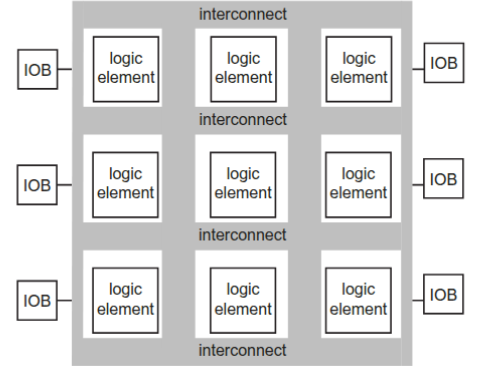
\includegraphics[width=0.6\linewidth]{Imagenes/03/03-FPGA_Fabrics.png} 
    \caption{Estructura genérica de la FPGA.}   
    \label{Fig:03-FPGA_Fabric}
\end{figure}
Estos tres elementos se combinan como puede verse en la \cref{Fig:03-FPGA_Fabric}, en los que los pines interaccionan con los elementos de lógica combinacional a través de las interconexiones. La lógica combinacional está dividida en unidades pequeñas, conocidas como \textbf{elementos de lógica} (LEs, \textit{logic elements}) o \textbf{bloques de lógica combinacional} (CLBs, \textit{combinational logic blocks}). Los LE o CLB pueden llegar a actura como las típicas puertas lógicas, claro que con na potencia mucho menor que la que podríamos encontrar en un bloque lógico combinacional encontrados en diseños grandes. Las interaconexiones se encuentran entre los elementos lógicos, y se programan (se selque tieneneccionan cuales están activas y cuales no). La interconexión suele estar organizada en canales u otras unidades. Los FPGAs normalmente ofrecen diferentes tipso de interconexiones dependiendo de la distancia entre los elementos lógicos combinacionales que tienen que conectarse. Las señales de reloj también son transportadas a través de su propia red de interconexión. Los pines I/O se llaman en general \textbf{bloques I/O} (IOBs). Estos también son programables, seleccionando si queremos que sean \textit{inputs} o \textit{ouputs}, y a veces cumplen objetivos tales como conexiones de baja potencia o alta velocidad. 

\begin{figure}[H] \centering
    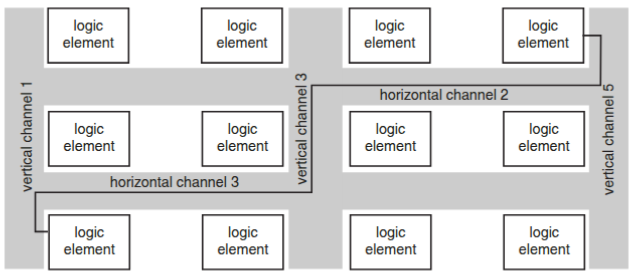
\includegraphics[width=0.6\linewidth]{Imagenes/03/03-FPGA_Interconexion.png} 
    \caption{Estructura genérica de la FPGA.}   
    \label{Fig:03-FPGA_Interconexion}
\end{figure}
Un diseñador de FPGAs debe estar dispuesto a usar diseños de conexiones preestablecidos, no como un diseñador VLSI que dibuja directamente las conexiones. El sistema de interconexión en los FPGAs suele ser uno de sus aspectos más complejos, debido a su cableado como propiedad global del diseño lógico. En la \cref{Fig:03-FPGA_Interconexion} se puede ver como sucede la interconexión entre elementos lógicos a través de un cambino complicado entre diferntes canales elegido por el diseñador.

Las conexiones entre elementos lógicos require caminos complejos debido a que los elementos lógicos LEs están dispuestos en una especie de estructura dos dimensional, por lo que las conexiones no solo son entre LEs, sino entre cables también. Los cables se organizan en tods tipos principales, los \textbf{canales cableados} y los \textbf{canales de ruta}. Los primeros corren los canales horizontales y los segundos los verticales. El diseñador es el que elige cual será usado para transportar la señal. 

Para poder permitir al diseñador lógico hacer todas las conexiones deseadas entre elementos lógicos, los canales FPGA deben estar provistos de cables de varios tamaños. Normalmente se usa la \textbf{estructura segmentada}, dado que cada cable esta formada por difernetes secciones de varias llongitudes. 

Todas las FPGAs necesitan ser programadas o configuradas. Existen tres tipos principales de FPGAs (tres tecnologías de circuitos): SRAM, \textit{antifuse} (antifusible) y \textit{flash}. No importa el tipo de circuito usado, los elementos principales de las FPGAs (lógica, interconexión, pines I/O) necesita ser configurada. Algunas de las características de interés para un diseñador que quiere usar un FPGA suele ser: 

\begin{itemize}
    \item ¿Cuánta lógica puede entrar en un FPGA? 
    \item ¿Cuantos pines I/O tengo? 
    \item ¿Cómo de rápido corre? 
\end{itemize}
Mientras que podemos determinar facilmente cuantos pines I/O tenemos, determinar la cantidad de lógica que podemos implementar y cuán rápido lo va a hacer es mucho más complicado. 



\section{FPGA basadas en SRAM}

Los FPGAs con memoria estática es uno de los más usados. 


\subsection{Elementos lógicos}

El método básico utilizado para construir un \textbf{bloque de lógica combinacional} (CLB), también llamado \textbf{elemento lógico} (LE), en un FPGA basado en SRAM es la \textbf{tabla de búsqueda} (LUT), cuyo esquema se puede ver en la \cref{Fig:03-LUT}. La tabla de búsqueda es una SRAM que se usa para implementar una tabla de verdad. Cada dirección en la SRAM representa una combinación de entradas del elemento lógico. El valor almacenado en esa dirección representa el valor de la función para esa combinación de entradas de n variables. Una función de n entradas requiere una SRAM con $2^n$ posiciones. Dado que una SRAM básica no está sincronizada con un reloj, la tabla de búsqueda (LE) opera como cualquier otra puerta lógica: a medida que cambian sus entradas, su salida cambia tras un cierto retraso.

\begin{figure}[H] \centering
    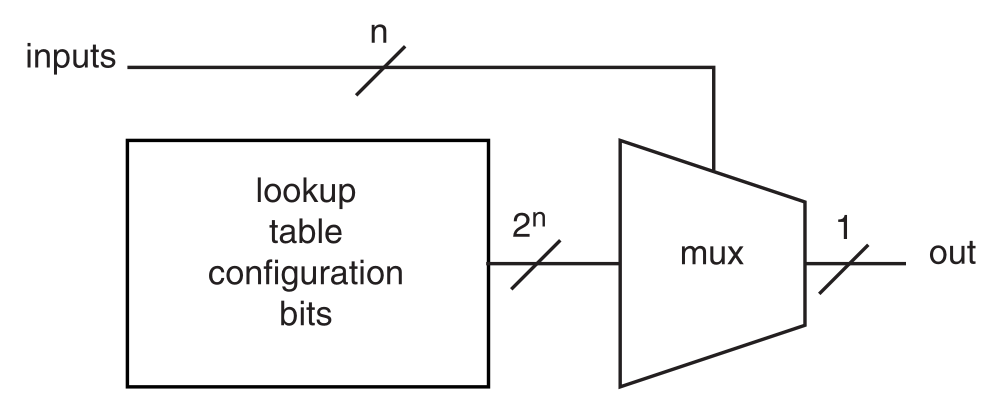
\includegraphics[width=0.6\linewidth]{Imagenes/03/03-LUT.png}
    \caption{esquema de una tabla de búsqueda (LUT).}
    \label{Fig:03-LUT}
\end{figure}

La razón por la que una función lógica de $n$ entradas necesita una SRAM con $2^n$ localizaciones es que cada combinación posible de los $n$ bits de entrada debe estar asociada a una salida determinada. Dado que cada entrada puede ser 0 o 1, el número total de combinaciones diferentes de $n$ bits es $2^n$ y, por lo tanto, para cubrir todas las posibilidades, la memoria necesita al menos $2^n$ direcciones (localizaciones). Cada dirección almacena la salida correspondiente a una combinación particular de entradas, permitiendo así implementar cualquier función booleana de $n$ entradas al usar las entradas como dirección en la memoria y leer la salida almacenada en esa dirección. Supongamos una función de 3 entradas $A$, $B$, $C$. Entonces $n=3$, y el número de localizaciones necesarias es
$$
2^3=8.
$$
Las combinaciones posibles de entrada y su dirección en la SRAM serían:

\[
\begin{array}{c c c | c}
A & B & C & \text{Dirección (binario)} \\
\hline
0 & 0 & 0 & 000 \\
0 & 0 & 1 & 001 \\
0 & 1 & 0 & 010 \\
0 & 1 & 1 & 011 \\
1 & 0 & 0 & 100 \\
1 & 0 & 1 & 101 \\
1 & 1 & 0 & 110 \\
1 & 1 & 1 & 111 \\
\end{array}
\]

Cada combinación corresponde a una localización de la SRAM: por ejemplo, si $A=0$, $B=1$, $C=0$, la combinación es 010 en binario, lo que corresponde a la dirección 2 (en decimal) de la SRAM, donde se almacena el valor de salida deseado para esa combinación.


A diferencia de una puerta lógica típica, la función representada por el LE (elemento lógico) puede cambiarse modificando los valores de los bits almacenados en la SRAM. Como resultado, un LE de n entradas puede representar $2^{2^n}$ funciones (aunque algunas de estas funciones son permutaciones entre sí). Un elemento lógico típico tiene cuatro entradas.

El retardo a través de la tabla de búsqueda (lookup table) es independiente de los bits almacenados en la SRAM, por lo que el retardo del elemento lógico es el mismo para todas las funciones. Esto significa que, por ejemplo, un LE basado en una tabla de búsqueda exhibirá el mismo retardo para una XOR de 4 entradas y para una NAND de 4 entradas. En contraste, una XOR de 4 entradas construida con lógica CMOS estática es considerablemente más lenta que una NAND de 4 entradas. Por supuesto, la puerta lógica estática es, en general, más rápida que el LE.

Los elementos lógicos generalmente contienen registros—flip-flops y latches—además de lógica combinacional. Un flip-flop o latch es pequeño comparado con el elemento de lógica combinacional (en marcado contraste con la situación en VLSI personalizado), por lo que tiene sentido añadirlo al elemento de lógica combinacional. Usar una celda separada para el elemento de memoria simplemente consumiría recursos de enrutamiento. Así los fabricantes pueden optimizar el ruteo local: el resultado de la LUT puede registrarse justo al lado, evitando que la señal viaje a bloques separados para sincronizarse, reduciendo tiempos de propagación. Además, los flip-flops permiten que el bloque lógico mantenga valores entre ciclos de reloj, posibilitando lógica secuencial. Si solo necesitas lógica combinacional, tu circuito produce salidas que dependen únicamente de sus entradas actuales, pero si quieres que tu circuito “recuerde” lo que pasó antes —es decir, que su comportamiento dependa no solo de las entradas actuales, sino también de entradas pasadas— necesitas almacenar estados (así obtenemos una \textit{lógica secuencial}). Esto se hace a través de \textit{flip-flops} y \textit{latches}.


También son posibles bloques lógicos más complejos. Por ejemplo, muchos elementos lógicos también contienen circuitería especial para la suma. Muchas FPGAs incorporan lógica especializada para sumadores dentro del elemento lógico. El componente crítico de un sumador es la cadena de acarreo (\textit{carry chain}), que puede implementarse de manera mucho más eficiente en lógica especializada que usando técnicas estándar basadas en tablas de búsqueda. Podemos ver la definción de acarreo en \cref{Sec:A-Acarreo}. 

Los ejemplos siguientes describen los elementos lógicos en dos FPGAs. Estos ejemplos ilustran tanto las similitudes entre las estructuras de FPGAs como los enfoques variados en el diseño de los elementos lógicos.


\vspace*{1em}

\begin{Ejemplo}
\subsection*{Ejemplo 3.1: Elementos lógicos Xlinx Spartan-II}
\end{Ejemplo}

En la \cref{Fig:03-Xilinx-Spartan-II} vemos el bloque lógico combinacional Xilinx Spartan II. Una slice incluye dos celdas lógicas (LCs). La base de una celda lógica es el par de tablas de búsqueda de cuatro bits. Sus entradas son F1-F4 y G1-G4. Cada tabla de búsqueda también puede usarse como una memoria RAM síncrona de 16 bits o como un registro de desplazamiento de 16 bits. Cada \textit{slice}\footnote{Un slice es como un mini-bloque lógico que puedes programar para implementar una pequeña parte de tu diseño: una puerta lógica, un bit de un registro, una parte de un sumador, etc.}  (LUTs, flip-flops..) también contiene lógica de acarreo para cada LUT, de modo que se puedan realizar sumas. Un acarreo de entrada al slice ingresa por la entrada CIN, pasa a través de los dos bits de la cadena de acarreo, y sale por COUT. La lógica aritmética también incluye una puerta XOR. Para construir un sumador, la puerta XOR se usa para generar la suma y la LUT se usa para el cálculo del acarreo. Cada slice incluye un multiplexor que se utiliza para combinar los resultados de los dos generadores de funciones en un slice. Otro multiplexor combina las salidas de los multiplexores en los dos slices, generando un resultado para todo el CLB.

Los registros pueden configurarse como flip-flops tipo D o como latches. Cada registro tiene señales de reloj y habilitación de reloj. Cada CLB también contiene dos drivers de tres estados (conocidos como BUFTs) que pueden usarse para manejar buses internos del chip.

\begin{figure}[H] \centering
    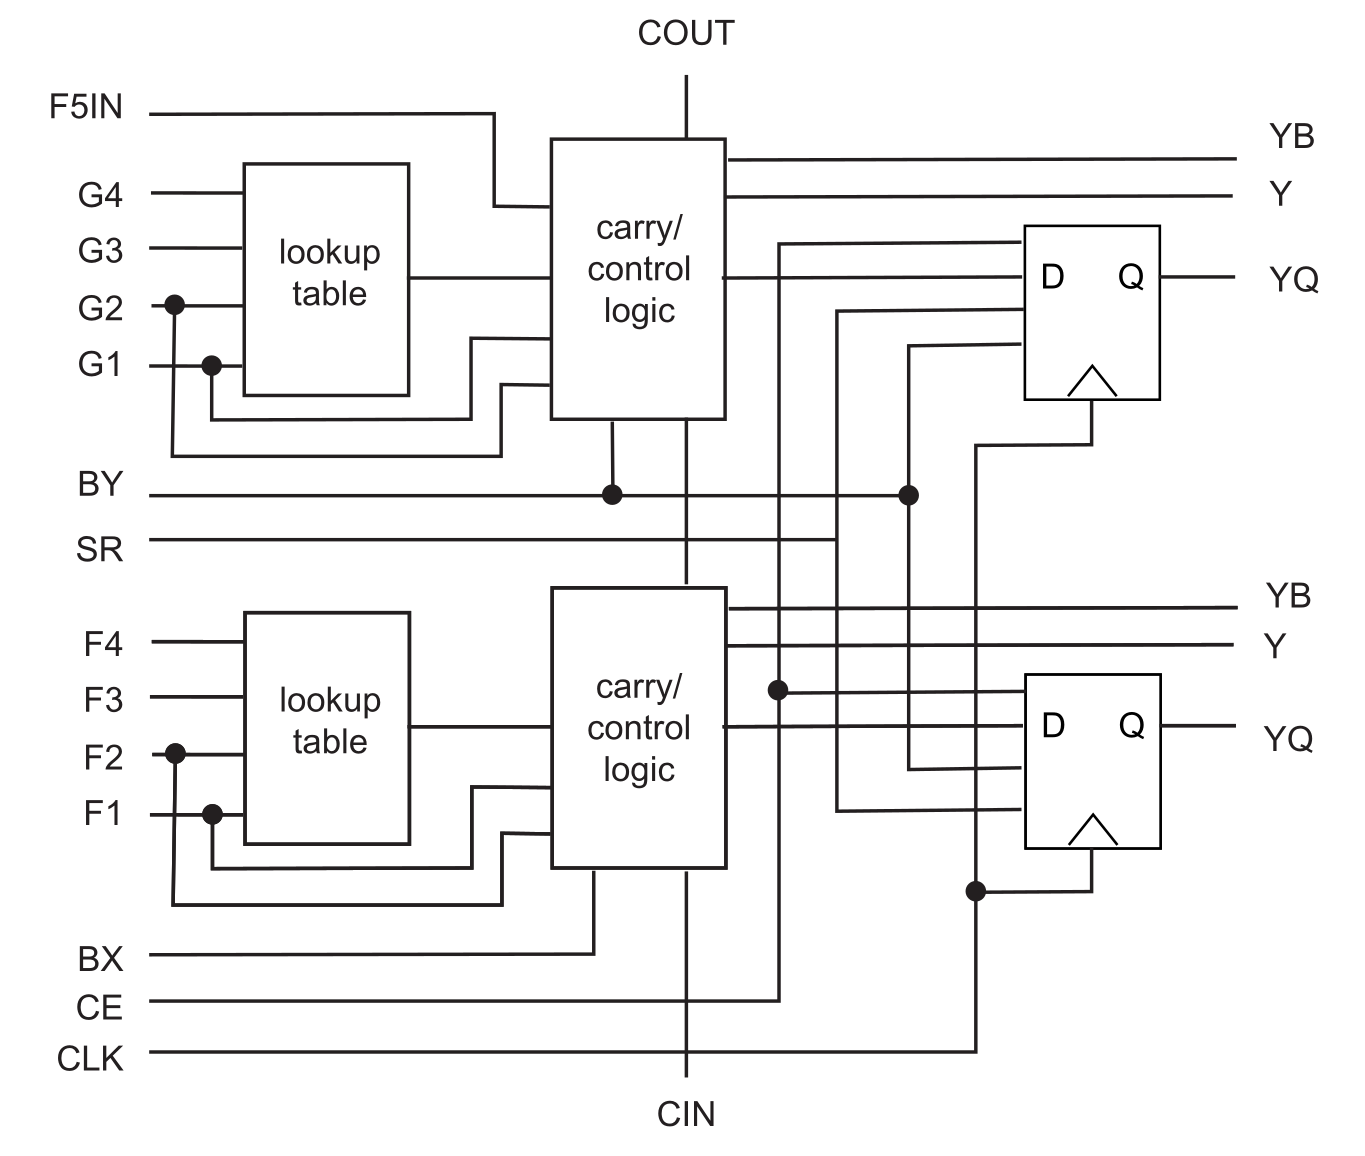
\includegraphics[width=0.6\linewidth]{Imagenes/03/03-Xilinx_Spartan_II.png}
    \caption{Elementos lógicos Xilinx Spartan II}%\cite{FPGA-WolfWayne}.}
    \label{Fig:03-Xilinx-Spartan-II}
\end{figure}

\vspace*{1em}

\begin{Ejemplo}
\subsection*{Ejemplo 3.2: Elementos lógicos Altera APEX II}
\end{Ejemplo}


\subsection{Redes interconectadas}